\section{Prioritering}
\subsection{Forretningsmæssige Betydning}
% MoSCW: I hvor høj grad er kravet forretningsmæssigt kritisk?
Til prioriteringen af brugsmønstrene er MoSCoW metoden benyttet. Resultatet kan ses nedenfor på figur \ref{fig:moscow}.\\

\begin{figure}[h]
\centering
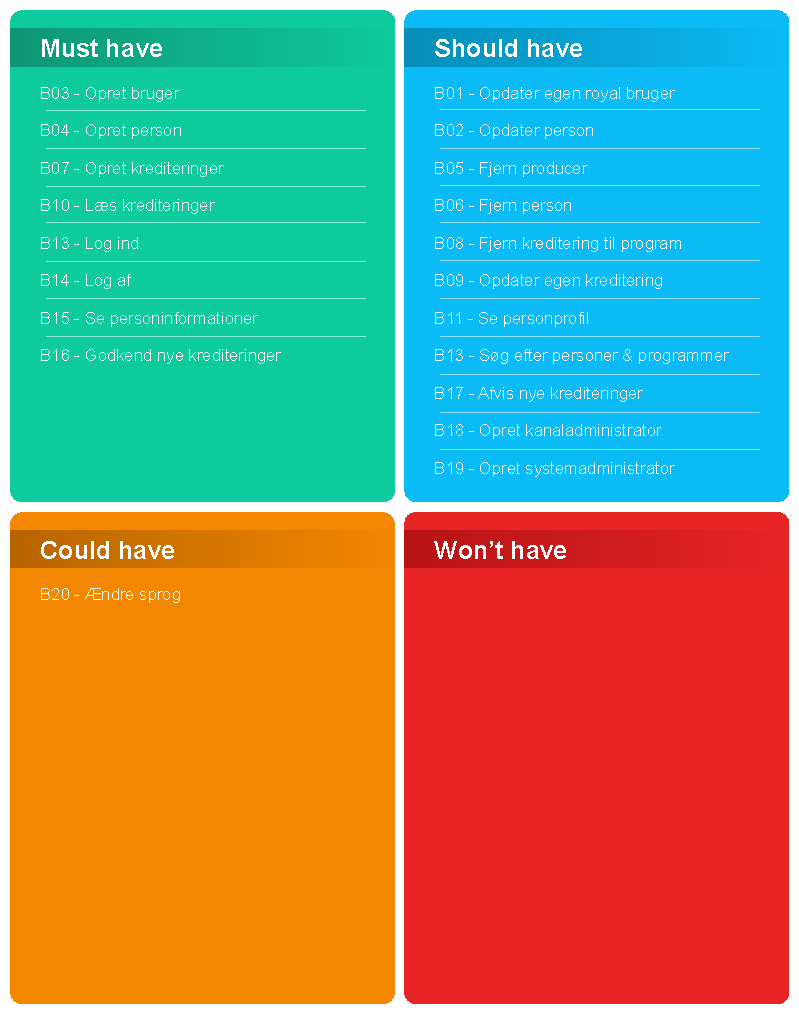
\includegraphics[scale=1]{figures/MoSCoW.pdf}
\caption{MoSCoW}
\label{fig:moscow}
\end{figure}

\noindent
Her ses de forskellige brugsmønstre I en MoSCoW. MoSCoW bruges til at finde ud af hvad der skal udvikles først. 
Da der ikke blev fundet ting i Inceptionsfasen, som der ikke skulle med dennegang, kom der ikke noget i "Won't have" sektionen.

\subsection{Arkitektonisk Betydning}

\noindent
De arkitektoniske krav der har en arketeknoisk betydning for systemet er:
\begin{itemize}
    \item Brugergrænsefladen til klienterne vil være på Dansk.
    \item Brugergrænsefladen(Swagger UI) til REST Api'et vil være på Engelsk.
    \item Persistens vil blive håndteret af en database
    \item Databasen vil være PostgreSQL
    \item Systemet vil automatisk starte efter evt. server genstart.
\end{itemize}
% Hvis vi arbejder med dette krav, vil det så i særlig grad hjælpe os til at få udviklet en passende løsningsstruktur?
% Som jeg forstår dette, bør vi se på alle vores funktionelle/ikke funktionelle krav, hvis kravet bidrager til en bedre løsningsstruktur, angiv kravet og fortæl hvordan.


%\subsection{Risiko} UNDLADET
% Hvis vi arbejder med dette krav, vil det så i særlig grad hjælpe os med at få håndteret risici?
% Som jeg forstår dette, bør vi se på alle vores funktionelle/ikke funktionelle krav, hvis kravet mindsker risici, nævn det.

\subsection{Læringsmæssige Udbytte}
% Hvis vi arbejder med dette krav, vil vi så i særlig grad opnå et læringsmæssigt udbytte?
% Som jeg forstår dette, bør vi se på alle vores funktionelle/ikke funktionelle krav, hvis kravet giver os en særlig grad af læringsmæssigt udbytte.
\begin{itemize}
    \item Supplerende krav - REST Api
    \begin{itemize}
        \item Vi har lagt op til et system der vil afspejle den løsning som TV2 oprindeligt lagde op til. Den løsning indeholder et REST Api, som er vurderet som værende udenfor det der forventes at kunne som studerende på nuværende tispunkt. Ved at vælge sådan en løsning, vil det give os et rigtigt godt redskab i vores programmerings-værktøjskasse i fremtidige projekter.
    \end{itemize}{}
\end{itemize}


\subsection{X-faktor}
% Handler dette krav om noget som vi vil finde særligt motiverende, spændende, sjovt ... at arbejde med?
\begin{itemize}
    \item \myworries{Der mangler reference til funktionkrav 14 - doobelt klip på mig og kig ned}
    \item \hyperref[table:funktionskrav]{K14 - Importering af data} 
    \begin{itemize}
        \item Integrationen mellem andre systemer, og gå de forskellige systemer til at spille sammen er spændende. Det er her med til at give systemet et løft, da det automatiserer oprettelsen af nye programmer i systemet.
    \end{itemize}{}
\end{itemize}

